\chapter{常用物理常数}
\href{https://en.wikipedia.org/wiki/List_of_physical_constants}{物理常数表}
\section{SI单位制}
\paragraph{基本单位}
\begin{notecaptionblock}
	\captionof{table}{SI基本单位}
	\begin{tabular}{ccc}
		\toprule
		物理量&单位&定义\\
		\midrule
		时间&\unit{\second}&$^\ast$\\
		长度&\unit{\metre}&光速$c$\\%和s\\
		质量&\unit{\kilogram}&Planck常数$h$\\%和m, s\\
		电流&\unit{\ampere}&元电荷$e$\\%和s\\
		热力学温度&\unit{\kelvin}&Boltzmann常数$\kB$\\%和kg, m, s\\
		物质的量&\unit{\mole}&Avogadro常数$\NA$\\
		发光强度&\unit{\candela}&$^{\ast\ast}$\\
		\bottomrule
	\end{tabular}
\end{notecaptionblock}
$^\ast\enspace$基态$\nuclide{133}{Cs}$超精细能级跃迁频率$\nu=\qty{9192631770}{Hz}$\\
\noindent
$^{\ast\ast}\enspace f=\qty{540E12}{Hz}$的单色辐射源辐射强度为$\frac1{683}\,\unit{\watt\per\steradian}$
\paragraph{词头}
\begin{notecaptionblock}
	\captionof{table}{SI词头}
	\begin{tabular}{ccc|ccc}
		\toprule
		名称&符号&系数&名称&符号&系数\\
		\midrule
		十&da&$10^1$&分&d&$10^{-1}$\\
		百&h&$10^2$&厘&c&$10^{-2}$\\
		千&k&$10^3$&毫&m&$10^{-3}$\\
		兆&M&$10^6$&微&\textmu&$10^{-6}$\\
		吉&G&$10^9$&纳&n&$10^{-9}$\\
		太&T&$10^{12}$&皮&p&$10^{-12}$\\
		拍&P&$10^{15}$&飞&f&$10^{-15}$\\
		艾&E&$10^{18}$&阿&a&$10^{-18}$\\
		泽&Z&$10^{21}$&仄&z&$10^{-21}$\\
		尧&Y&$10^{24}$&幺&y&$10^{-24}$\\
		\bottomrule
	\end{tabular}
\end{notecaptionblock}
\paragraph{导出单位}
\begin{notecaptionblock}
	\captionof{table}{SI导出单位}
	\begin{tabular}{ccc}
		\toprule
		物理量&单位&基本单位表达\\
		\midrule
		角&\unit{\radian}&$1$\\
		立体角&\unit{\steradian}&$1$\\
		频率&\unit{\hertz}&\unit{\per\second}\\
		力&\unit{\newton}&\unit{\kilogram\metre\per\second\squared}\\
		压强&\unit{\pascal}&\unit{\kilogram\per\metre\per\second\squared}\\
		能量、功&\unit{\joule}&\unit{\kilogram\metre\squared\per\second\squared}\\
		功率、辐射通量&\unit{\watt}&\unit{\kilogram\metre\squared\per\second\cubed}\\
		电荷&\unit{\coulomb}&\unit{\ampere\second}\\
		电压&\unit{\volt}&\unit{\kilogram\metre\squared\per\ampere\per\second\cubed}\\
		电容&\unit{\farad}&\unit{\ampere\squared\second\tothe{4}\per\kilogram\per\metre\squared}\\
		电阻&\unit{\ohm}&\unit{\kilogram\metre\squared\per\ampere\squared\per\second\cubed}\\
		电导&\unit{\siemens}&\unit{\ampere\squared\second\cubed\per\kilogram\per\metre\squared}\\
		电感&\unit{\henry}&\unit{\kilogram\metre\squared\per\ampere\squared\per\second\squared}\\
		磁通量&\unit{\weber}&\unit{\kilogram\metre\squared\per\ampere\per\second\squared}\\
		磁感应强度&\unit{\tesla}&\unit{\kilogram\per\ampere\per\second\squared}\\
		温差（摄氏度）&\unit{\degreeCelsius}&\unit{\kelvin}\\
		光通量&\unit{\lumen}&\unit{\candela}\\
		照度&\unit{\lux}&\unit{\candela\per\metre\squared}\\
		放射性活度&\unit{\becquerel}&\unit{\per\second}\\
		\bottomrule
	\end{tabular}
\end{notecaptionblock}
\section{SI单位制定义的准确值}
\begin{compactitem}
	\item 真空中光速
		\begin{align}
			c:=\qty{299792458}{\metre\per\second}.
		\end{align}
	\item Planck常数
		\begin{align}
			h:=\qty{6.62607015E-34}{\joule\second}
		\end{align}
		约化Planck常数
		\begin{align}
			\hbar:=\frac{h}{2\pi}=\qty{1.05457182E-34}{\joule\second}.
		\end{align}
	\item 电荷单位(elementary charge)
		\begin{align}
			e:=\qty{1.602176634E-19}{C}.
		\end{align}
		电子伏与焦耳的换算为 $\qty{1}{eV}=\qty{1.602176634e-19}{J}$。
	\item Boltzmann常数
		\begin{align}
			\kB:=\qty{1.380649E-23}{\joule\per\kelvin}.
		\end{align}
	\item Avogadro常数
		\begin{align}
			\NA:=\qty{6.02214076E23}{\per\mole}.
		\end{align}
\end{compactitem}
\paragraph{由定义推导出的准确物理常数}~
\begin{compactitem}
	\item 理想气体常数
		\begin{align}
			R:=\kB\NA=\qty{8.314462618}{\joule\per\kelvin\per\mole}
		\end{align} % 15324
	\item Faraday常数
		\begin{align}
			F:=\NA e=\qty{9.648533212E4}{\coulomb\per\mole}
		\end{align} % 33100184
	\item Stefan--Boltzmann常数
		\begin{align}
			\sigma:=\frac{2\pi^5\kB^4}{15h^3c^2}=\qty{5.670374419E-8}{\watt\per\metre\squared\per\kelvin\tothe{4}}
		\end{align} % 184429453971
	\item Wien位移定律常数
		\begin{align}
			\lambda_{\max} T=\frac{hc}{\xi\kB}=\qty{2.897771955}{\milli\metre\kelvin}
		\end{align} % 185172661
		$\xi=\num{4.965114232}\ldots$是方程$\xi=5(1-\e^{-\xi})$的解。
	\item 第一辐射常数(first radiation constant)
		\begin{equation}
			c_1=2\pi hc^2=\qty{3.741771852E-16}{\watt\metre\squared}.
		\end{equation} % 192758011367103884
	\item 第二辐射常数(second radiation constant)
		\begin{equation}
			c_2=\frac{hc}\kB=\qty{1.4387768775E-2}{\metre\kelvin}.
		\end{equation} % 03933802146671602
\end{compactitem}
\section{常用的物理常数}
\sisetup{uncertainty-mode = compact}
\begin{itemize}
	\item 万有引力常数(gravitational constant)
		\begin{align}
			G=\qty{6.67430(15)e-11}{\metre\cubed\per\kilogram\per\second\squared}
		\end{align}

	\item 真空介电常数(permittivity of free space)
		\begin{align}
			\varepsilon_0=\qty{8.8541878128(13)E-12}{\farad\per\metre};
		\end{align}
		真空磁导率(permeability of free space)
		\begin{align}
			\mu_0=\qty{1.25663706212(19)E-6}{\henry\per\metre};
		\end{align}
		一个非常接近的值是旧SI单位制下用来定义安培（\unit{A}）的$\mu_0$
		\[
			\mu_0:=4\pi\times 10^{-7}\,\unit{\henry\per\metre},
		\]
		自由空间阻抗(impedance of free space)
		\begin{equation}
			Z_0:=\sqrt{\frac{\mu_0}{\varepsilon_0}}=\qty{376.730313412(59)}{\ohm}
		\end{equation}
		由于$c=1/\sqrt{\varepsilon_0\mu_0}$；有近似值$Z_0=\mu_0c\simeq 120\pi\,\unit{\ohm}.$

	\item 精细结构常数(fine-structure constant)
		\begin{align}
			\alpha:={}&\frac{e^2}{4\pi\varepsilon_0}\frac1{\hbar c}=\num{7.2973525693(11)E-3};\\
			\alpha^{-1}={}&\num{137.035999084(21)}.
		\end{align}

	\item 原子质量单位
		\begin{align}
			\qty{1}{u}=\frac{M(\nuclide{12}{C})}{12}=\qty{1.66053906660(50)E-27}{kg}.
		\end{align}
		一个非常接近的值是旧SI单位制下Avogadro常数的定义：
		\[
			\qty{1}{u}=\frac1{\NA}\,\unit{g}.
		\]

	\item 电子、质子、中子质量
		\begin{align}
			m_\electron&=\qty{9.1093837015(28)E-31}{kg}\\
			&=\qty{5.48579909065(16)E-4}{u}\\
			&=\qty{0.51099895000(15)}{MeV}/c^2.\\
			m_\proton&=\qty{1.67262192369(51)E-27}{kg}\\
			&=\qty{1.007276466621(53)}{u}\\
			&=\qty{938.27208816(29)}{MeV}/c^2;\\
			m_\neutron&=\qty{1.67492749804(95)E-27}{kg}\\
			&=\qty{1.00866491588(49)}{u}\\
			&=\qty{939.56542052(54)}{MeV}/c^2.
		\end{align}
		质子电子质量比
		\begin{align}
			\frac{m_\proton}{m_\electron}=\num{1836.15267343(11)}.
		\end{align}
		电子荷质比
		\begin{align}
			\frac e{m_\electron}=\qty{1.75882E11}{\coulomb\per\kilogram}.
		\end{align}

	\item 电子Compton波长和约化Compton波长
		\begin{align}
			\lambda_\electron&=\frac h{m_\electron c}=\qty{2.42631023867(73)}{pm};\\
			\lambdabar_\electron&=\frac{\lambda_\electron}{2\pi}=\qty{3.861 592 6796(12)E-13}{m}.
		\end{align}

	\item 经典电子半径
		\begin{align}
			r_\electron:=\frac{e^2}{4\pi\varepsilon_0}\frac1{m_\electron c^2}=\alpha\lambdabar_\electron=\qty{2.8179403262(13)}{fm}
		\end{align}
		Thomson散射截面
		\begin{align}
			\sigma_\electron:=\frac{8\pi}3r_\electron^2=\qty{6.6524587321(60)E-29}{\metre\squared}.
		\end{align}



	\item Bohr半径
		\begin{align}
			a_0:=\frac{4\pi\varepsilon_0}{e^2}\frac{\hbar^2}{m_\electron}=\frac{r_\electron}{\alpha^2}=\qty{5.29177210903(80)E-11}{m}.
		\end{align}
	\item Rydberg常量
		\begin{align}
			R_\infty:=\frac{\alpha^2}{2\lambda_\electron}=\qty{10973731.568160(21)}{\per\metre}
		\end{align}
		Rydberg单位能量
		\begin{align}
			\qty{1}{Ry}:=\frac{e^2}{4\pi\varepsilon_0\cdot 2a_0}=\qty{2.1798723611035(42)e-18}{J}
		\end{align}

	\item Bohr磁子
		\begin{align}
			\muB:=\frac{e\hbar}{2m_\electron}=\qty{9.2740100783(28)E-24}{\joule\per\tesla}
		\end{align}
\end{itemize}
\paragraph{常用常数组合}
\begin{align}
	hc&=\qty{1.986445857E-25}{\joule\metre}\\ % 14892870
	&=\qty{1.239841984E-6}{\electronvolt\metre}\\  % 332002622377527446
	\hbar c&=\qty{3.161526773E-26}{\joule\metre}\\ % 496689987889773799
	&=\qty{1.97326980459E-7}{\electronvolt\metre}\\ % 3024658908971331
	\frac{e^2}{4\pi\varepsilon_0}&=\qty{2.307077552E-28}{\joule\metre}\\ % 341736287791637868
	&=\qty{1.4399645478E-9}{\electronvolt\metre} % 42567205852558868
\end{align}
$\qty{1}{eV}$对应频率
\begin{equation}
	\nu_0=\frac eh=\qty{2.417989242E14}{Hz}
\end{equation} % 084918162238291425
$\qty{1}{eV}$对应波数
\begin{equation}
	k_0=\frac e{hc}=\qty{8.065543937E5}{\per\metre}
\end{equation} % 349211641069007231

\chapter{元素周期表}

\begin{figure}[h]
	\centering
	\tikzfigure[width=\linewidth]{periodic-table}
	\caption{元素周期表}
	\label{fig:periodic_table}
\end{figure}

ref: \href{https://texample.net/tikz/examples/periodic-table-of-chemical-elements}{Periodic Table of Chemical Elements}.

All Credit to Ivan Griffin.

\chapter{放射系}

三图以质子数 $Z$ 为横轴、中子数 $N$ 为纵轴。沿箭头从母核读向子核，$\alpha$ 衰变使质子数和中子数各减少 2，$\beta^-$ 衰变则使质子数增加 1、中子数减少 1。
箭头的线宽表示分支比，颜色按本页的对数色标表示该条衰变记录的半衰期。同一核素的不同能态共用一个格点，例如 $\nuclide{234\mathrm{m,g}}{Pa}$ 中的 $\mathrm m$ 和 $\mathrm g$ 分别表示异能态和基态。同质异能跃迁画成自环。若同一对母、子核素有多条记录，图上仅保留原程序最后读入的一条。各分支比对应各自的初态，$\mathrm{m,g}$ 标记本身不提供两个态的布居比例。

\begin{figure}[!htbp]
	\centering
	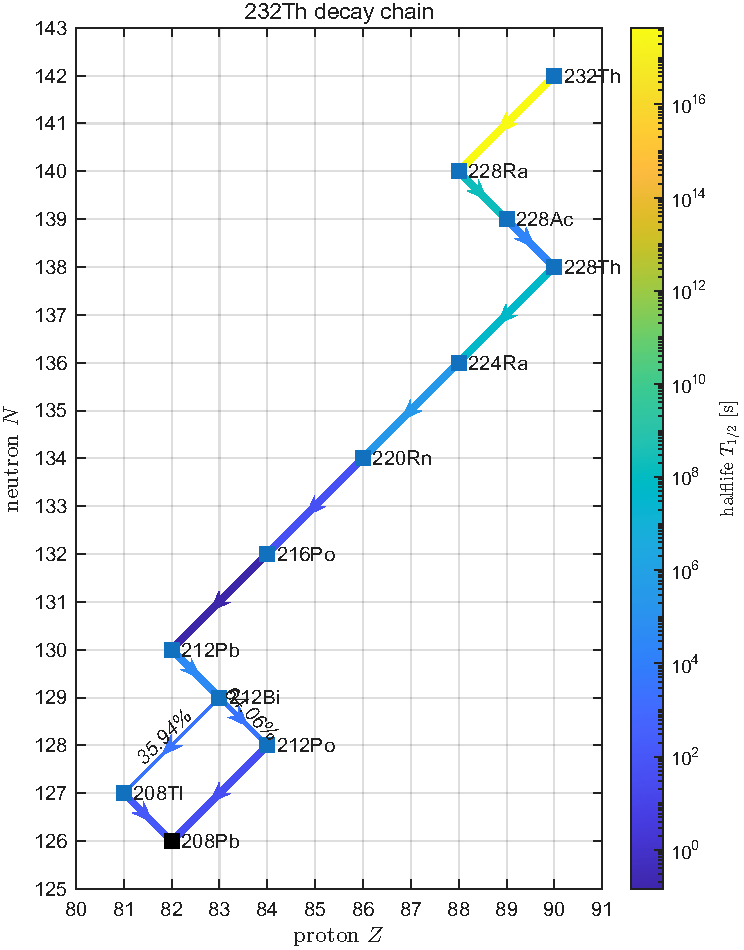
\includegraphics[page=1,height=.57\textheight]{figures/decay_system.pdf}
	\caption{钍系$\nuclide{232}{Th}$衰变图}
	\label{fig:decay_system 232Th}
\end{figure}

\begin{figure}[hp]
	\centering
	\includegraphics[page=2]{figures/decay_system.pdf}
	\caption{铀系$\nuclide{238}{U}$衰变图}
	\label{fig:decay_system 238U}
\end{figure}

\begin{figure}[hp]
	\centering
	\includegraphics[page=3]{figures/decay_system.pdf}
	\caption{锕铀系$\nuclide{235}{U}$衰变图}
	\label{fig:decay_system 235U}
\end{figure}



% \printindex
